\begin{exo}
  \donnee{Dans sa tournée, un voyageur de commerce doit se rendre de la ville A à la ville B. Il dispose de deux itinéraires : le premier en passant par la ville C et le second par la ville D. Aucune liaison directe entre A et B existe.  Les temps en heures (h) que passe sur la route le voyageur de commerce pour se déplacer de A à B via les villes C et D peuvent être représentés par des variables aléatoires indépendantes $X_1,X_2,X_3,X_4$ définies par
  \begin{enumerate}
  	\item $X_1$ : "Durée du trajet entre les villes A et C";
  	\item $X_2$ : "Durée du trajet entre les villes C et B";
  	\item $X_3$ : "Durée du trajet entre les villes A et D";
  	\item $X_4$ : "Durée du trajet entre les villes D et B";
  \end{enumerate}
On suppose que ces variables aléatoires sont toutes issues d'une distribution normale. Les temps espérés pour se déplacer d'une ville à l'autre se trouvent dans la figure ci-dessous et le coefficient de variation de chacune de ces variables aléatoires vaut 0.2.
\begin{center}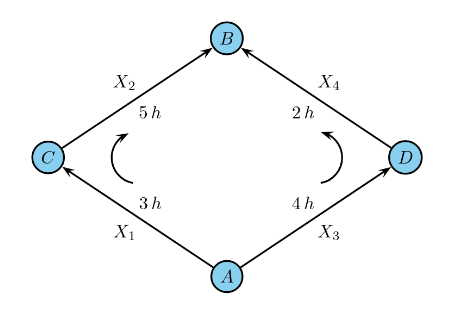
\includegraphics[scale=0.8]{ex5}\end{center}
}
	\begin{subexo}{Le coefficient de variation $\delta_X$ d'une variable aléatoire X est donné par $\frac{\sigma_X}{\mu_X}$. Calculer les écarts-type des variables $X_1,X_2,X_3,X_4$.}
		\begin{center}
			Premièrement, $\delta = \frac{\sigma}{\mu} \iff \sigma = \mu \cdot \delta$. Comme, $\delta = 0.2$, nous déduisons pour chaque distribution:
			  \begin{enumerate}
				\item $\sigma_1$ : $\mu_1 \cdot 0.2 = 0.6$ 
				\item $\sigma_2$ : $\mu_2 \cdot 0.2 = 0.1$ 
				\item $\sigma_3$ : $\mu_3 \cdot 0.2 = 0.8$ 
				\item $\sigma_4$ : $\mu_4 \cdot 0.2 = 0.4$ 
			\end{enumerate}
		Dès lors, nous pouvons décrire chaque distribution comme:
		  \begin{enumerate}
			\item $X_1 \sim \N\left(3, (0.6)^2\right)$
			\item $X_2 \sim \N\left(5, (1)^2\right)$
			\item $X_3 \sim \N\left(4, (0.8)^2\right)$
			\item $X_4 \sim \N\left(2, (0.4)^2\right)$
		\end{enumerate}
		\end{center}
	\end{subexo}	
	\begin{subexo}{Calculer la probabilité que le trajet entre la ville A et B via C dure moins de 9 heures.}
		\begin{center}
			Définissons: $T_1 = X_1 + X_2 \sim \N(\mu_1 + \mu_2, \sigma_1^2 + \sigma_2^2) = \N(8,1.36)$
		\end{center}
		\begin{align*}
			P(A \rightarrow B \rightarrow C \leq 9) &= P(X_1 + X_2 \leq 9) \\
			&= P(T_1 \leq 9) \\
			&= P\left(\frac{T_1-8}{\sqrt{1.36}} \leq \frac{9-8}{\sqrt{1.36}}\right) \\
			&= \phi(0.86) \approx 0.9
		\end{align*}
	\end{subexo}
	\begin{subexo}{Déterminer la probabilité que la durée du trajet entre A et B via C soit plus courte que celle via D en considérant la varible aléatoire $T = T_1 - T_2$ ou $T_1$ représente la durée du trajet via C et $T_2$ celle du trajet via D.}
	\end{subexo}
	\begin{center}
		Commençons par calculer $T_2$ de la même manière que $T_1$, \\
		$T_1 \sim \N\left(8,0.6^2 + 1^2\right) = \N(8,1.36)$ \\
		$T_2 \sim \N\left(6,0.4^2 + 0.8^2\right) = \N(6,0.8)$ \\
		Alors, (attention pas évident)\\
		$T = T_1 - T_2 \sim \N\left(8-6, 1.36 + 0.8\right) = \N(2,2.16)$
	\end{center}
		Ensuite, centrons et réduisons la probabilité cherchée $P(T < 0)$ sans oublier de centrer réduire.
		\begin{align*}
			P(T < 0) & = P\left(\frac{T-2}{\sqrt{2.16}} \leq \frac{-2}{\sqrt{2.16}}\right) \\
			&\approx \phi(-1.36) \\
			&= 1- \phi(1.36) \\
			&\approx 0.087
		\end{align*}
\end{exo}
